% !TeX spellcheck = da_DK
\section{Systembeskrivelse} 
Dette afsnit indeholder en beskrivelse af det biofeedbacksystem, der skal kunne anvendes af patienter som et træningsapparat i rehabiliteringen af balanceproblemer. Systembeskrivelsen indeholder målgruppen for designet samt, hvilket formål og anvendelse det har. Ud fra disse faktorer er systemet blevet designet og illustreret i et blokdiagram. 

\subsection{Systemets bruger}
Systemet udvikles til patienter med balanceproblemer mhp. selvtræning af balance i rehabiliteringsfase $3$ og $4$ jævnfør afsnit \ref{Faser}, side \pageref{Faser}. Systemet skal være let anvendeligt, da det udvikles til anvendelse i hjemmet af patienterne selv. Systemets design skal altså være simpelt, så der ikke skabes forvirring blandt patienterne ift. funktionerne. Fagkyndigt personale, såsom fysioterapeuter og læger, skal kunne instruere patienten i brugen af systemet samt følge med i den udvikling, patienterne gennemgår. Det skal derfor være muligt for det fagkyndige personale at anvende systemet og aflæse data herfra. 
%Dette gøres ved at have et analogt og digitalt output, hvor den digitale del henvender sig til det fagkyndige personale i form af grafer, mens den analoge del henvender sig til apopleksipatienterne. \fxnote{Erikas kommentar: relevans ift. analogt og digitalt output? Tekniske detaljer! Er det vigtigt, at det er et analog output eller at det output indeholder specifik information?}   

\subsection{Systemets formål og anvendelse}\label{formaal_anvendelse}
Systemets input er patienternes kropshældning i det frontale plan, dvs. hvor meget vedkommende svajer under udførelse af forskellige balanceøvelser. % i stående udgangsposition, som er beskrevet i tredje punkt i afsnit \ref{rehabiliteringbalance} på side \pageref{rehabiliteringbalance}. 
Systemet skal kunne konvertere informationer vedrørende patienternes kropshældning til visuel og somatosensorisk feedback samt et digitalt output i form af grafer. Den visuelle og somatosensoriske feedback har til formål at gøre patienterne opmærksomme på, hvornår de har bevæget sig ud i en risikozone for fald. Således kan systemet registrere, hvis patienten er i risiko for at falde. Når patienten bevæger sig ud i en risikozone, udsendes feedback, så patienterne har mulighed for at rette sig op. Selve systemet skal anvendes til selvtræning i hjemmet ved udførelse af balanceøvelser, der træner den stående balance. Det skal derfor være et brugervenligt system og skal kunne påsættes uden problemer og fungere uden, at patienten skal navigere rundt i forskellige funktioner. Systemet skal fungere som en hjælp for patienten, da vedkommende bliver bevidst omkring sin balance.% Herved kan apopleksipatienten være mere selvstændig i rehabiliteringsprocessen.
%Patienterne kan anvende systemet ved to sværhedsgrader ift. kropsposition: normal kropsstilling (anatomisk udgangsposition) og ovenstående omtalte øvelse. %Apopleksipatienternes balance udfordres i højere grad af SRT end ved normal kropsstilling, eftersom kropsvægten fordeles anderledes ved denne øvelse ift. den normale kropsstilling omtalt i afsnit \ref{BalanceAfsnit} på side \pageref{BalanceAfsnit}. 
%SRT udføres i stående udgangsposition med fødderne på en tegnet linje, så den ene fods tæer er mod den anden fods hæl. Derudover holdes armene tæt ind til kroppen og over kors. \cite{Huo1999}.\fxnote{Erikas rettelser til dette skal tilføjes}\\ %Denne position er valgt for at udfordre patientens balance ved at fordele kropsvægten anderledes ift. den normale kropsstilling omtalt i afsnit \ref{BalanceAfsnit} på side \pageref{BalanceAfsnit}. % Patienten påsætter selv systemet øverst på sternum og udfører herefter en kort prøvetest for at kende til de givne feedback parametre.Under prøvetesten svajer patienten langsomt fra side til side. 
%Det er på baggrund af afsnit \ref{MekBioFeed} på side \pageref{MekBioFeed} valgt at hældningen på patienten skal opfanges vha. et accelerometer, der er placeret øverst på sternum. 

Jævnfør afsnit \ref{MekBioFeed}, side \pageref{MekBioFeed} er det valgt, at systemet skal placeres øverst på sternum for at få bedst mulige målinger ift. patienternes kropshældning. Systemet skal give visuel og somatosensorisk feedback i form af fem LED'er, bestående af en grøn, to gule og to røde, samt to vibratorer. Med denne metode indikeres både, hvilken retning patienten svajer samt graden heraf. Ved benyttelse af to feedbackformer kan en større patientgruppe anvende systemet. Hvis f.eks. patientens visuelle sans er begrænset, kan systemet stadig benyttes grundet den somatosensorisk feedback. Jævnfør afsnit \ref{BalanceAfsnit}, side \pageref{BalanceAfsnit} er grænsen for, hvornår et fald forekommer ift. hældningsgrad individuel. I praksis bør systemet dermed tilpasses den enkelte patient på baggrund af testøvelser ift. balancen. %Hældningsgraderne vil i dette projekt blive valgt på baggrund af raske forsøgspersoner, da det vurderes udfra problemanalysen afsnit \ref{BalanceAfsnit}, side \pageref{BalanceAfsnit}, at patienter har flere sygdomsrelaterede faktorer, der kan påvirke deres hældningsgrad. 

%Hvis patienten hælder i intervallet $8^{\circ}$-$13^{\circ}$ til højre, indikeres dette af den gule diode på højresiden af den grønne diode. Derudover aktiveres en mild vibration mod patientens hænder, når den gule diode lyser. Hvis patienten hælder $13^{\circ}$ eller derover, lyser den røde diode til højre for den gule diode og styrken af vibrationen forøges. Det samme gør sig gældende for hældning mod venstre. Med denne metode indikeres både, hvilken retning patienten svajer samt graden heraf. Ved benyttelse af to feedback former er der større mulighed for, at patienten kan opfange signalerne. Hvis patientens visuelle sans er begrænset kan systemet stadig benyttes grundet den somatosensorisk feedback. \\ 

For at øge øvelsernes sværhedsgrad kan den visuelle sans udelukkes. Patienten skal under øvelser forsøge at holde balancen så længe som muligt uden at bevæge sig ud i risikozonerne. Hvis patienten kommer ud i en risikozone, vil dette blive markeret ved lys i LED'erne samt vibration. Træningsøvelser gentages efter behov. Ved at tage flere målinger igennem rehabiliteringsforløbet vil det forventes, at der sker en fremgang ift. tiden, hvori balancen kan opretholdes uden at patienten bevæger sig ud i risikozonerne. 

\subsection{Accelerometer}\label{Subsec:AccTeori}
Det valgte accelerometer af typen ADXL335, som fremgår af \figref{ADXL335}, er en treakset sensor, som kan anvendes til måling af statisk balance. Den har dimensionerne $2$x$2$x$0.2$ i cm.  

\begin{figure}[H]
	\centering 
	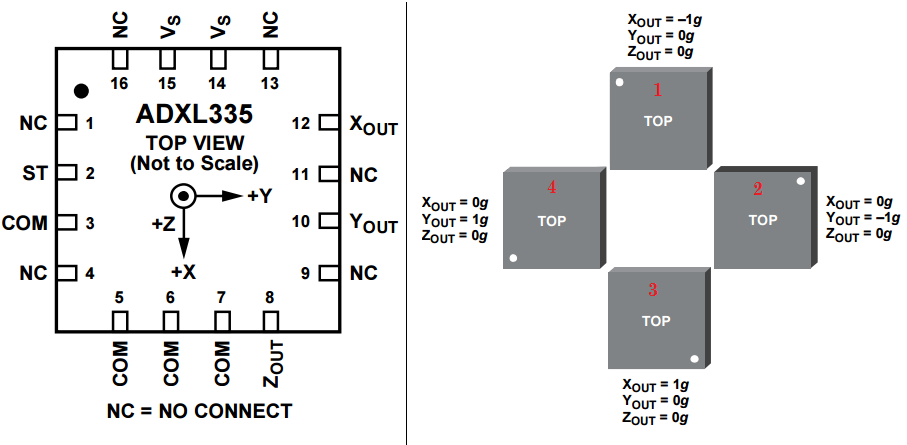
\includegraphics[scale=0.5]{figures/cProblemloesning/ADXL335_2.JPG}
	\caption{På figuren ses accelerometeret af typen ADXL335 i forskellige stillinger. Til venstre på figuren ses accelerometerets pin konfiguration og funktions beskrivelse. Til højre ses hvordan accelerometret skal placeres for forskellig g påvirkning. \textit{(Revideret)} \cite{Devices2009}}
	\label{ADXL335}
\end{figure}

\noindent Accelerometeret har en single-supply spændingsforsyning, der skal ligge mellem $1.8$ - $3.6$V. På accelerometeret er en regulator tilkoblet, som forhindrer en spændingsforsyning på over $3.3$V.  Arbejdsområdet ligger mellem $\pm3.6$g, og outputtet fra accelerometeret er maksimalt på $\pm1.188$V ift. accelerometerets indbyggede offset. Offsettet varierer efter spændingsforsyningen, men ligger ved $3$V forsyning på $1.5$V og beregnes ved $Off = Vs/2$. Båndbredden for x- og y-akserne ligger mellem $0.5$ til $1,600$Hz og for z-aksen mellem $0.5$ til $550$Hz. Støjen fra $X_{out}$ og $Y_{out}$ ligger normalt på $150\mu g/\sqrt{Hz}$ RMS, mens det for $Z_{out}$ ligger på $300\mu g/\sqrt{Hz}$ RMS. Denne enhed\fxnote{betyder, at den spektrale effekttæthed måles i $\mu g$ og dividerer dette med kvadratroden af båndbredden for signalet $\sqrt{Hz}$, hvilket} giver RMS af accelerationsstøjen ved en temperatur på $25^\circ$C. Sensitiviteten afhænger, ligesom offsettet, af spændingsforsyningen, da accelerometeret er ratiometrisk\fxnote{NTK: Ratiometrisk vil sige, at output er direkte proportionelt med input.} og ligger ved $3$V forsyning på $300 mV/g$ med en tolerance på $\pm10\%$. Accelerometerets outputimpedans er $32K\Omega$ med en afvigelse på $\pm15\%$. \cite{Devices2009} %Outputtet ligger normalt ved -1.08g i X-aksen og  1.08g Y-aksen og 1.83 g ved Z-aksen. 

Når accelerometeret hældes til siden, vil en acceleration ske ift. tyngdekraften i en given retning, og dermed sker et udslag i volt fra referencepunktet ved en hældning på $0^{\circ}$. Hvis accelerometeret placeres i stilling $1$, som det fremgår til højre på \figref{ADXL335}, påvirkes x-aksen med $-1$g.\cite{Devices2009} \\
På baggrund af sammenhængen mellem de enkelte parametre, der udtrykkes ved nedenstående ligninger, kan patientens hældning bestemmes.
\begin{align}
	V_{out} = V_{offset} + sensitiviteten \cdot tyngdekraften \cdot \sin(vinklen) \\
	V_{out} = V_{offset} + \frac{\Delta V}{\Delta g} \cdot g \cdot \sin \Theta
\end{align}

\subsection{Overordnede funktionelle krav til systemet}\label{FunkKrav}
\begin{itemize}
	\item Systemet skal være simpelt, så det kan anvendes af patienter og fagkyndigt personale.
	\item Systemet skal kunne måle kropshældning, samt angive i hvilken retning hældningen sker. 
	\item Systemet skal kunne give visuel og somatosensorisk feedback ved forskellige hældningsgrader.
	\begin{itemize}
		\item Grøn LED: Skal lyse, når patienten ikke er ude i risikozonerne og informere patienten om, at accelerometeret er placeret korrekt.  
		\item Gul LED: Skal lyse, når den første risikozone defineret i grader indtræffer og slukke, hvis patienten retter sig op.
		\item Rød LED: Skal lyse, når den anden risikozone defineret i grader indtræffer og slukke, hvis patienten retter sig op.
		\item Vibration: Skal aktiveres, når den første risikozone indtræffer, dvs. aktiveres samtidig med den gule LED, og skal slukke, hvis patienten retter sig op.
	\end{itemize}
	\item Systemet skal kunne give et digitalt output, så fagkyndigt personale kan aflæse og gemme patienternes data.
\end{itemize}

\subsection{Systemets opbygning}\label{ref:blokdiagram}
Systemets opbygning fremgår af \figref{kravblok}.

\begin{figure}[H]
	\centering
	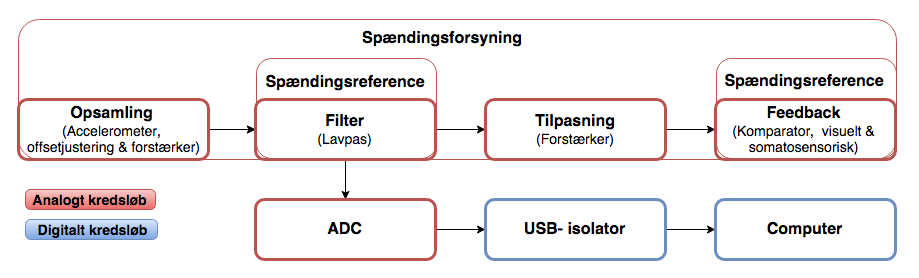
\includegraphics[scale=0.73]{figures/cProblemloesning/blokdiagram.PNG}
	\caption{På figuren ses et blokdiagram med de enkelte blokke, som systemet skal indeholde.}
	\label{kravblok}
\end{figure}
Det biologiske signal, der opsamles med accelerometeret, skal som det første centreres omkring $0$V ved en offsetjustering og efterfølgende forstærkes. Herefter skal signalet filtreres for at frasortere uønskede signaler, der ligger uden for signalets spektrum. Efterfølgende deles systemet i en analog og digital del. I den analoge del følger en tilpasning af signalet i form af en forstærkning. Efterfølgende sendes signalet over i en feedbackkonfiguration indeholdende komparatorer og feedbackkomponenter. Inputsignalet sammenlignes her med definerede tærskelværdier, der hver især er tilkoblet bestemte feedbackkomponenter, som skal udløses, hvis tærskelværdien overskrides. Tærskelværdierne sættes ud fra bestemte hældningsgrader for accelerometret. \\
I den digitale del af systemet ledes signalet ind i en ADC. Denne konverterer det analoge biologiske signal til et digitalt signal. Det digitale signal ledes herefter ind i en USB-isolator for at øge patientens sikkerhed ved adskillelse mellem systemet og elnettet. Til sidst overføres det digitale signal til en computer, hvor det efterfølgende visualiseres som en graf og gemmes. \\
Systemet har dermed både et output henvendt til patienterne og det fagkyndige personale. Patienternes output er de feedbackkomponenter, der oplyser omkring deres hældningsgrad. Programmet, der behandler og gemmer patienternes øvelsesresultater, er output til det fagkyndige personale.

